\section{Hasil bilateral sepuluh mitra}\label{sec:bilateral}

\subsection{Perbedaan arah dan dukungan model}

Hasil bilateral membedakan satu hubungan agregat menjadi sepuluh pengalaman pasar. Tabel berikut memakai koefisien depresiasi NARDL dan window setelah holdback. Australia dan Malaysia memenuhi penyaringan level serta diagnostik utama, tetapi signifikansi keduanya tidak sama tahan terhadap BH. Model lain tetap dilaporkan walaupun mempunyai koefisien besar atau probabilitas kecil tanpa dukungan level lengkap.

\begin{table}[!htbp]\centering\caption{Ringkasan NARDL bilateral Indonesia}{\small\setlength{\tabcolsep}{3pt}\renewcommand{\arraystretch}{1.15}
\begin{tabular}{p{0.17\linewidth}p{0.045\linewidth}p{0.2\linewidth}p{0.12\linewidth}p{0.09\linewidth}p{0.09\linewidth}p{0.07\linewidth}}
\toprule
\textbf{Mitra} & \textbf{N} & \textbf{Rentang} & \textbf{Koef. dep.} & \textbf{p} & \textbf{BH} & \textbf{Status}\\
\midrule
Australia & 77 & 2007Q1--2026Q1 & 3,356 & \(<0{,}001\) & 0,004 & L+D\\
Tiongkok & 78 & 2007Q1--2026Q2 & -2,727 & 0,250 & 0,350 & --\\
India & 49 & 2014Q1--2026Q1 & -6,443 & 0,236 & 0,350 & --\\
Jepang & 78 & 2007Q1--2026Q2 & -2,456 & 0,006 & 0,020 & --\\
Korea Selatan & 78 & 2007Q1--2026Q2 & 3,935 & 0,144 & 0,288 & --\\
Malaysia & 78 & 2007Q1--2026Q2 & 1,346 & 0,024 & 0,059 & L+D\\
Singapura & 78 & 2007Q1--2026Q2 & -0,262 & 0,810 & 0,810 & --\\
Thailand & 78 & 2007Q1--2026Q2 & 0,950 & 0,280 & 0,350 & L\\
Amerika Serikat & 75 & 2007Q1--2025Q3 & 3,095 & 0,006 & 0,020 & --\\
Vietnam & 74 & 2007Q1--2025Q2 & -0,551 & 0,737 & 0,810 & --\\
\bottomrule
\end{tabular}
}\label{tab:bilateral}\end{table}

\begin{figure}[!htbp]\centering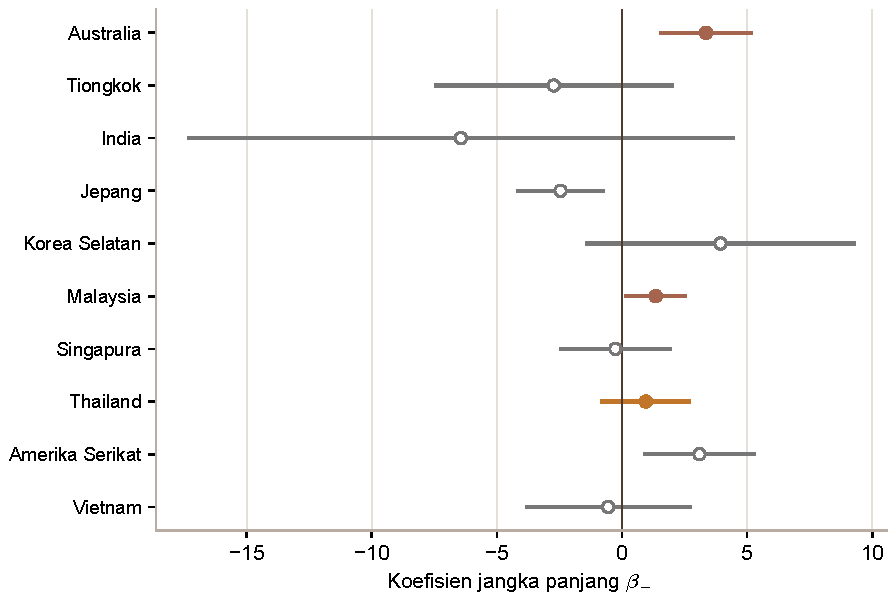
\includegraphics[width=\linewidth]{assets/bilateral_forest.pdf}\caption{Koefisien depresiasi bilateral NARDL. Warna cokelat menunjukkan L+D, emas L, dan simbol kosong dukungan level belum lengkap. Semua negara pada sumbu adalah mitra Indonesia.}\label{fig:bilateralforest}\end{figure}


Perbedaan antarmitra belum merupakan uji formal selisih koefisien pada sampel sama. India berawal lebih akhir, sedangkan AS dan Vietnam berakhir lebih awal. Regresi yang berbeda juga mengendalikan GDP dan kurs bilateral yang berbeda. Uraian tiap mitra berikut menghubungkan angka, status dan grafik agar penafsiran tidak bergantung pada satu kolom bintang.

\clearpage\subsection{Indonesia--Australia}

NARDL Indonesia--Australia memakai 77 kuartal pada 2007Q1--2026Q1. Koefisien depresiasi 3,356, CI nominal 95\% [1,563; 5,149], probabilitas nominal \(<0{,}001\), dan BH 0,004. Probabilitas asimetri jangka panjang 0,147. Pemeriksaan yang membatasi: tidak ada penolakan pada penyaringan yang digunakan.

Australia menjadi contoh yang lebih mendukung perbaikan rasio neraca saat depresiasi. ARDL dan NARDL sama-sama memenuhi penyaringan level dan diagnostik. Koefisien depresiasi NARDL tetap signifikan setelah BH dalam keluarga bilateral, sedangkan Wald kesamaan apresiasi dan depresiasi tidak ditolak pada lima persen. Pemakaian NARDL karena itu tidak berarti asimetri pasti ditemukan.

Estimasi titik NARDL mempunyai pemburukan awal lalu perbaikan. Band awal masih melintasi nol, sehingga urutan J tidak terkonfirmasi sama kuat pada dua fase. Pernyataan yang lebih tepat adalah adanya pola J pada titik yang didukung kelayakan model, dengan ketidakpastian fase awal. Ini berbeda dari menyatakan depresiasi pasti menurunkan neraca pada kuartal pertama.

\begin{figure}[!htbp]\centering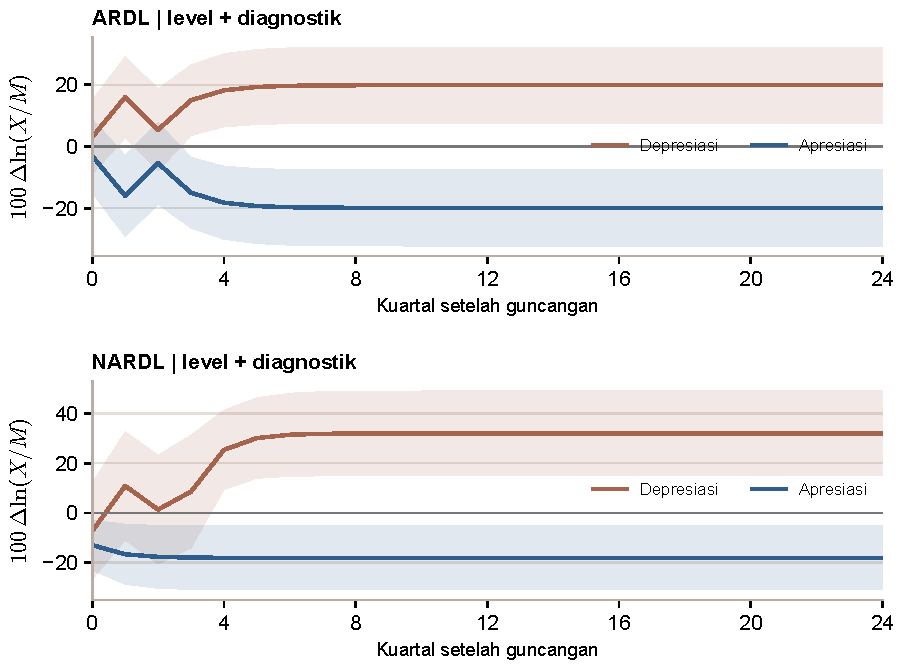
\includegraphics[width=\linewidth]{assets/response_BIL_AUS.pdf}\caption{Respons perdagangan Indonesia--Australia. Positif berarti perbaikan rasio ekspor/impor. Band pointwise nominal 95\%; skala kedua panel berbeda.}\label{fig:bilAUS}\end{figure}


\clearpage\subsection{Indonesia--Tiongkok}

NARDL Indonesia--Tiongkok memakai 78 kuartal pada 2007Q1--2026Q2. Koefisien depresiasi -2,727, CI nominal 95\% [-7,427; 1,972], probabilitas nominal 0,250, dan BH 0,350. Probabilitas asimetri jangka panjang 0,905. Pemeriksaan yang membatasi: F/t bounds belum menolak; joint-X belum menolak; catatan diagnostik residual/stabilitas.

Besarnya nilai perdagangan dengan Tiongkok tidak membuat koefisiennya otomatis paling presisi atau paling dapat ditafsirkan. Kedua model bilateral utama belum memenuhi syarat level lengkap. Pada NARDL terdapat catatan korelasi serial; pada ARDL CUSUM ditolak. Arah negatif belum dapat dipakai sebagai bukti jangka panjang bahwa depresiasi merugikan seluruh perdagangan Indonesia dengan Tiongkok.

Hasil kelompok pertanian dengan Tiongkok kemudian memberi gambaran yang lebih terukur. Perbedaan hasil total dan kelompok menandai peran agregasi, tetapi belum merupakan uji bahwa kedua koefisiennya berbeda secara statistik. Defisit bilateral yang besar pada statistik tahunan juga tidak mengidentifikasi sebab akibat dari perubahan kurs.

\begin{figure}[!htbp]\centering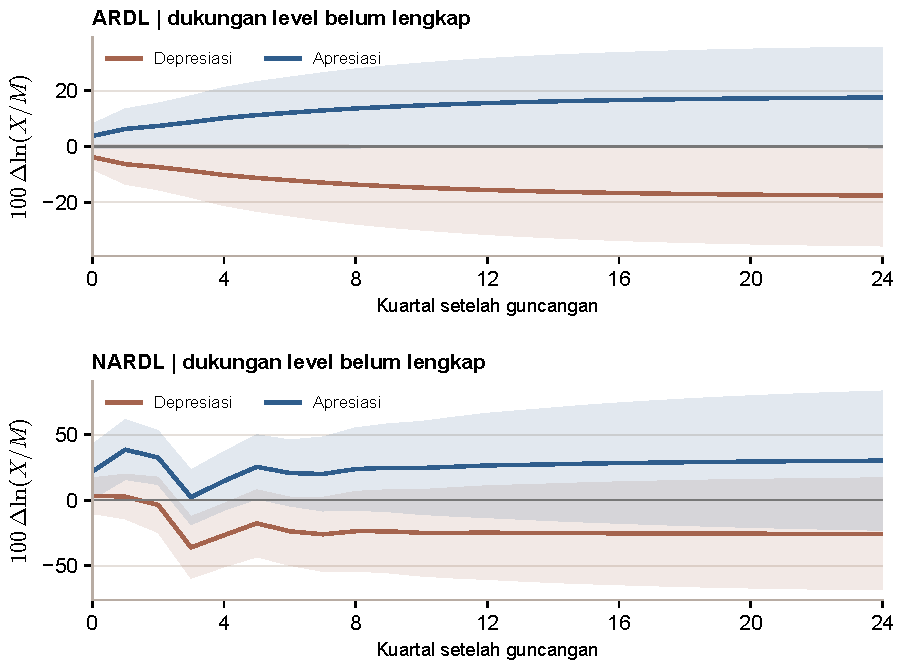
\includegraphics[width=\linewidth]{assets/response_BIL_CHN.pdf}\caption{Respons perdagangan Indonesia--Tiongkok. Positif berarti perbaikan rasio ekspor/impor. Band pointwise nominal 95\%; skala kedua panel berbeda.}\label{fig:bilCHN}\end{figure}


\clearpage\subsection{Indonesia--India}

NARDL Indonesia--India memakai 49 kuartal pada 2014Q1--2026Q1. Koefisien depresiasi -6,443, CI nominal 95\% [-17,300; 4,414], probabilitas nominal 0,236, dan BH 0,350. Probabilitas asimetri jangka panjang 0,021. Pemeriksaan yang membatasi: F/t bounds belum menolak; joint-X belum menolak.

India memakai sampel yang lebih pendek karena baseline menggunakan CPI mulai 2013. Dengan tambahan partial sums dan lag, ruang informasi per parameter menjadi terbatas. Koefisien depresiasi NARDL negatif tetapi intervalnya lebar; bounds belum mendukung level. Penolakan Wald asimetri tidak mengatasi masalah tersebut.

Model NARDL tidak ditolak pada penyaringan residual yang dipakai, sedangkan ARDL mempunyai catatan korelasi serial dan RESET. Ini contoh model yang residualnya tampak lebih mendukung tetapi hubungan levelnya belum memenuhi syarat. WPI menyediakan sensitivitas terpisah dengan konsep harga serta rentang yang berbeda; ia tidak diperlakukan sebagai CPI murni untuk memperpanjang baseline.

\begin{figure}[!htbp]\centering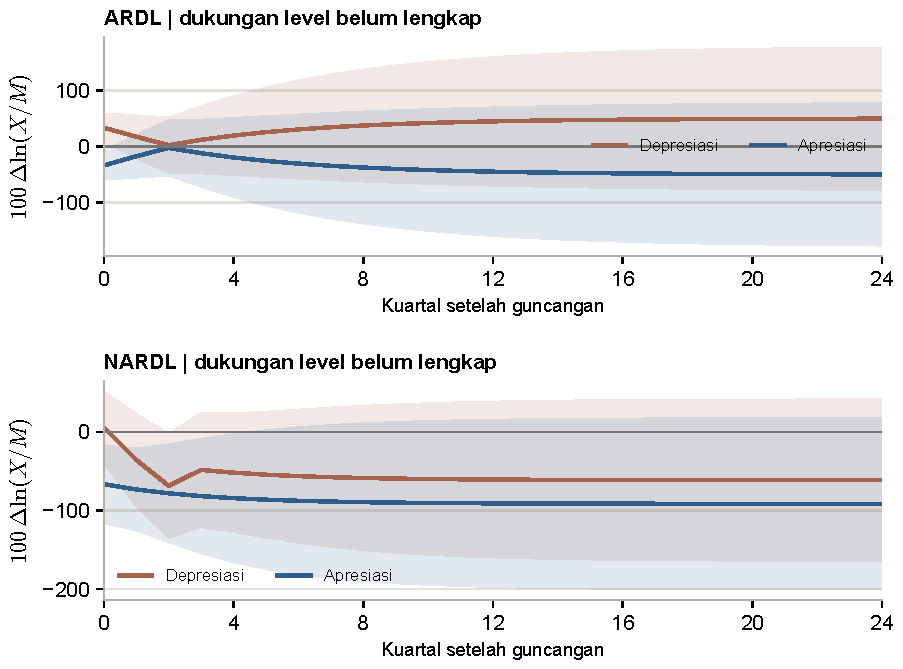
\includegraphics[width=\linewidth]{assets/response_BIL_IND.pdf}\caption{Respons perdagangan Indonesia--India. Positif berarti perbaikan rasio ekspor/impor. Band pointwise nominal 95\%; skala kedua panel berbeda.}\label{fig:bilIND}\end{figure}


\clearpage\subsection{Indonesia--Jepang}

NARDL Indonesia--Jepang memakai 78 kuartal pada 2007Q1--2026Q2. Koefisien depresiasi -2,456, CI nominal 95\% [-4,166; -0,747], probabilitas nominal 0,006, dan BH 0,020. Probabilitas asimetri jangka panjang 0,971. Pemeriksaan yang membatasi: F/t bounds belum menolak; catatan diagnostik residual/stabilitas.

Jepang memperlihatkan mengapa probabilitas koefisien saja dapat menyesatkan. Koefisien depresiasi NARDL negatif dan signifikan nominal maupun BH dalam keluarga bilateral. F upper bound menolak pada lima persen, tetapi t upper bound belum melewati ambang yang sama. Penyaringan hubungan level lengkap karena itu belum terpenuhi.

Selain itu, ARCH dan normalitas residual memberi catatan. Hasil ini tidak dihapus dari pelaporan, tetapi bobot penafsirannya berbeda dari kasus yang mendukung level dan diagnostik. Tanda negatif menjadi indikasi yang memerlukan peninjauan spesifikasi, bukan kesimpulan kausal mengenai respons ekspor Indonesia ke Jepang.

\begin{figure}[!htbp]\centering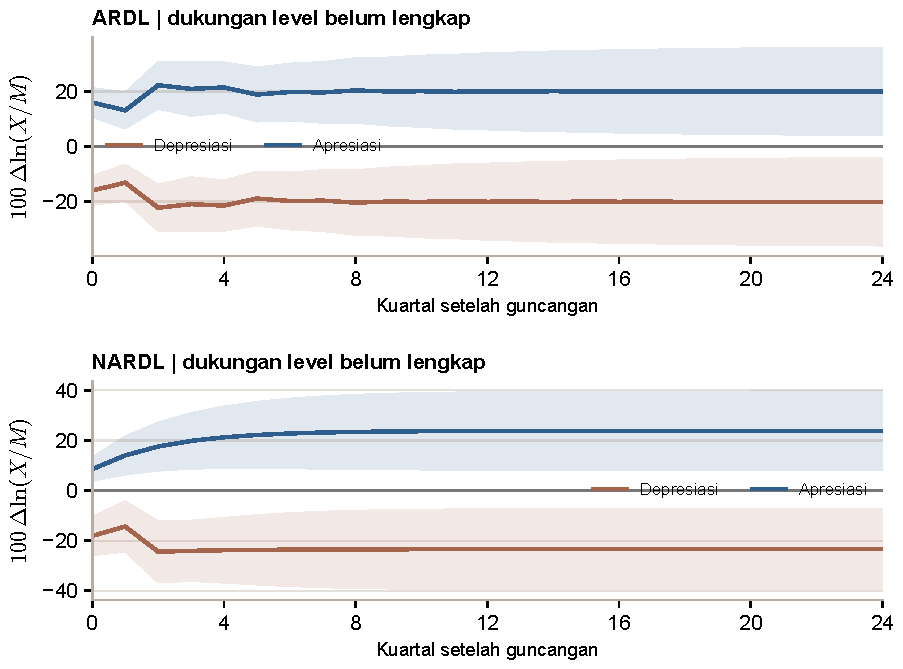
\includegraphics[width=\linewidth]{assets/response_BIL_JPN.pdf}\caption{Respons perdagangan Indonesia--Jepang. Positif berarti perbaikan rasio ekspor/impor. Band pointwise nominal 95\%; skala kedua panel berbeda.}\label{fig:bilJPN}\end{figure}


\clearpage\subsection{Indonesia--Korea Selatan}

NARDL Indonesia--Korea Selatan memakai 78 kuartal pada 2007Q1--2026Q2. Koefisien depresiasi 3,935, CI nominal 95\% [-1,383; 9,253], probabilitas nominal 0,144, dan BH 0,288. Probabilitas asimetri jangka panjang 0,112. Pemeriksaan yang membatasi: F/t bounds belum menolak; joint-X belum menolak; catatan diagnostik residual/stabilitas.

NARDL Korea menghasilkan koefisien depresiasi positif dengan ketidakpastian yang cukup besar. Dukungan level belum lengkap, dan korelasi serial, RESET serta CUSUM memberi catatan. ARDL lebih dekat ke nol tetapi juga belum mendukung level. Kedua hasil belum menetapkan bahwa efek nasional pada mitra ini kecil ataupun positif secara pasti.

Pada kelompok modal, NARDL mempunyai pola J yang lebih jelas dan lolos penyaringan utama. Kontras ini menunjukkan bahwa hasil agregat mitra dapat menyembunyikan respons kelompok tertentu. Kelompok modal tetap tidak mewakili semua ekspor ke Korea, dan band jalurnya masih bersifat pointwise.

\begin{figure}[!htbp]\centering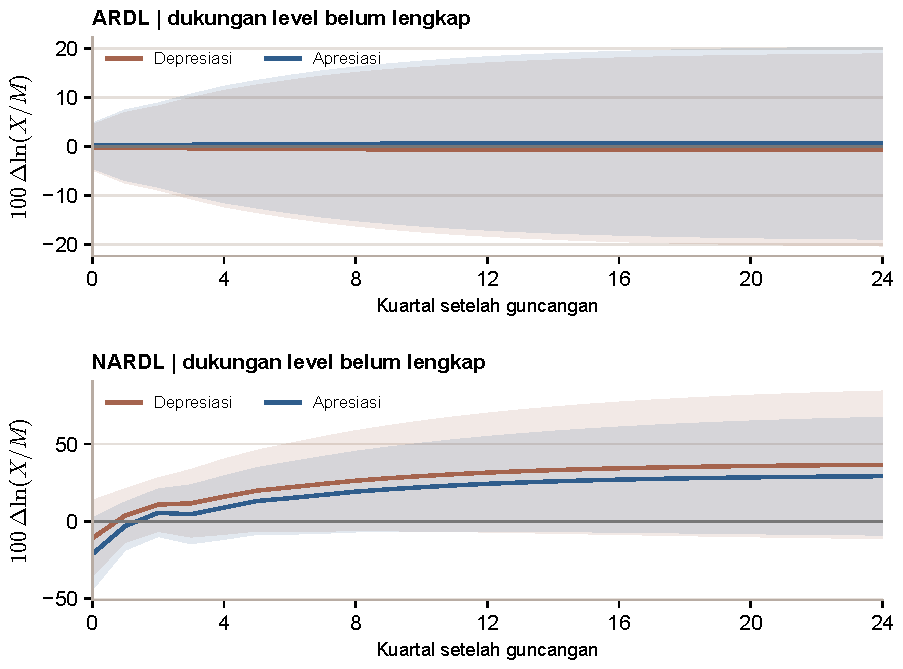
\includegraphics[width=\linewidth]{assets/response_BIL_KOR.pdf}\caption{Respons perdagangan Indonesia--Korea Selatan. Positif berarti perbaikan rasio ekspor/impor. Band pointwise nominal 95\%; skala kedua panel berbeda.}\label{fig:bilKOR}\end{figure}


\clearpage\subsection{Indonesia--Malaysia}

NARDL Indonesia--Malaysia memakai 78 kuartal pada 2007Q1--2026Q2. Koefisien depresiasi 1,346, CI nominal 95\% [0,186; 2,507], probabilitas nominal 0,024, dan BH 0,059. Probabilitas asimetri jangka panjang \(<0{,}001\). Pemeriksaan yang membatasi: tidak ada penolakan pada penyaringan yang digunakan.

Malaysia menunjukkan perbedaan yang nyata antara spesifikasi linier dan nonlinear. ARDL mempunyai dukungan level tetapi koefisien kursnya negatif, tidak signifikan pada lima persen, serta mempunyai catatan RESET dan CUSUM. NARDL memberi koefisien depresiasi positif, dukungan level dan diagnostik yang lebih baik, serta penolakan asimetri.

Probabilitas depresiasi NARDL sekitar 0,024 secara nominal, tetapi BH sekitar 0,059. Dengan demikian, klaim signifikansinya berubah menurut apakah pengujian berganda diperhitungkan. Respons yang cenderung membaik tidak harus diberi nama J-curve apabila fase awal yang memburuk tidak muncul. Temuan ini mendukung pembacaan perbaikan kondisional dengan ketahanan signifikansi yang terbatas.

\begin{figure}[!htbp]\centering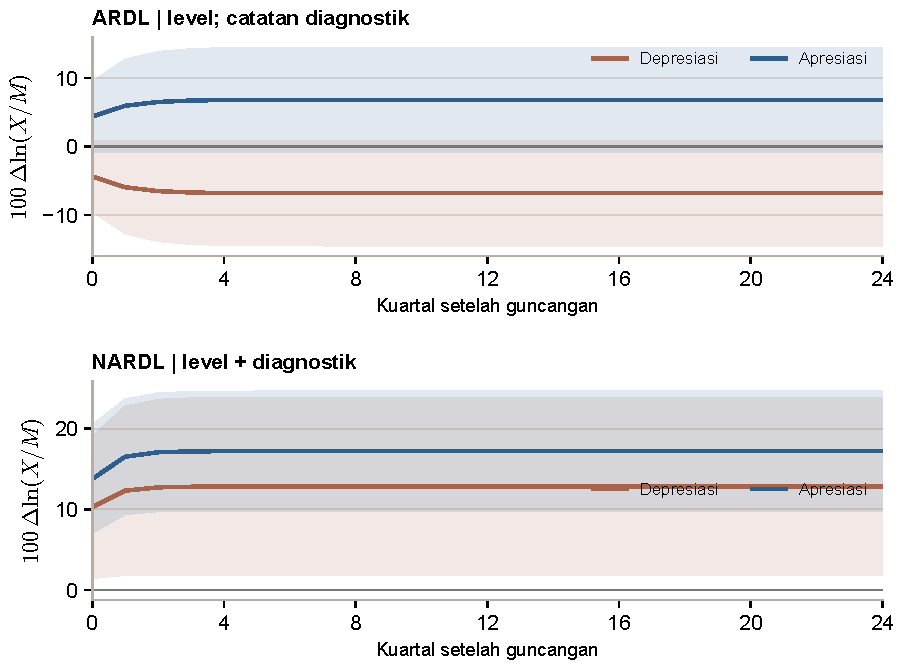
\includegraphics[width=\linewidth]{assets/response_BIL_MYS.pdf}\caption{Respons perdagangan Indonesia--Malaysia. Positif berarti perbaikan rasio ekspor/impor. Band pointwise nominal 95\%; skala kedua panel berbeda.}\label{fig:bilMYS}\end{figure}


\clearpage\subsection{Indonesia--Singapura}

NARDL Indonesia--Singapura memakai 78 kuartal pada 2007Q1--2026Q2. Koefisien depresiasi -0,262, CI nominal 95\% [-2,440; 1,915], probabilitas nominal 0,810, dan BH 0,810. Probabilitas asimetri jangka panjang 0,791. Pemeriksaan yang membatasi: joint-X belum menolak; catatan diagnostik residual/stabilitas.

Pada Singapura, F dan t bounds dapat menolak sementara joint-X tidak mendukung. Keputusan level lengkap karena itu tetap belum lolos. ARDL juga memberi contoh bahwa diagnostik yang tidak ditolak tidak cukup bila komponen level regressor belum terdukung. NARDL menambahkan catatan korelasi serial.

Koefisien depresiasi NARDL dekat nol dalam titik dibandingkan beberapa mitra lain, tetapi intervalnya tetap harus dibaca sebelum menyebut ketidakpekaan. Run ini tidak melakukan uji ekuivalensi efek kecil. Hasil yang paling dapat dipertahankan adalah belum adanya hubungan jangka panjang yang cukup didukung pada spesifikasi utama.

\begin{figure}[!htbp]\centering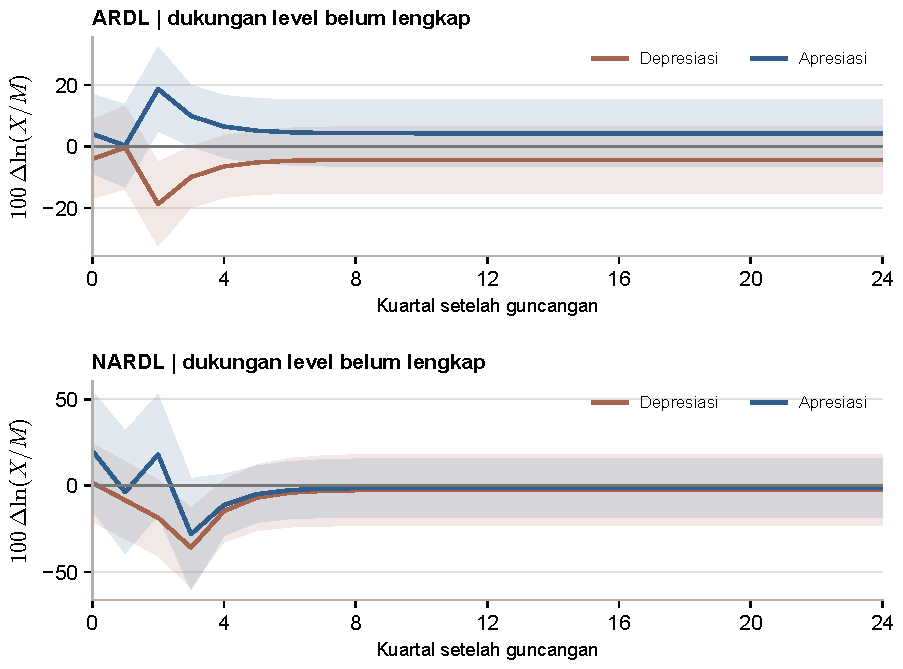
\includegraphics[width=\linewidth]{assets/response_BIL_SGP.pdf}\caption{Respons perdagangan Indonesia--Singapura. Positif berarti perbaikan rasio ekspor/impor. Band pointwise nominal 95\%; skala kedua panel berbeda.}\label{fig:bilSGP}\end{figure}


\clearpage\subsection{Indonesia--Thailand}

NARDL Indonesia--Thailand memakai 78 kuartal pada 2007Q1--2026Q2. Koefisien depresiasi 0,950, CI nominal 95\% [-0,789; 2,690], probabilitas nominal 0,280, dan BH 0,350. Probabilitas asimetri jangka panjang 0,765. Pemeriksaan yang membatasi: catatan diagnostik residual/stabilitas.

Thailand berbeda dari banyak pasangan karena kedua model memenuhi syarat level operasional. Namun ARCH dan CUSUMSQ ditolak, dengan tambahan CUSUM pada NARDL. Dukungan kointegrasi dan kestabilan residual karena itu tidak bergerak bersama. Koefisien positif NARDL juga belum signifikan secara nominal.

Kurs Thailand mempunyai catatan perbedaan konsep antarcompiler. Keluarga GEM dijalankan penuh sebagai sensitivitas, bukan digunakan untuk menambal satu observasi baseline. Perbandingan sumber tetap perlu memperhatikan apakah window dan definisinya sama. Sampai isu tersebut diperiksa lebih jauh, koefisien tidak dibaca sebagai efek kebijakan yang telah stabil.

\begin{figure}[!htbp]\centering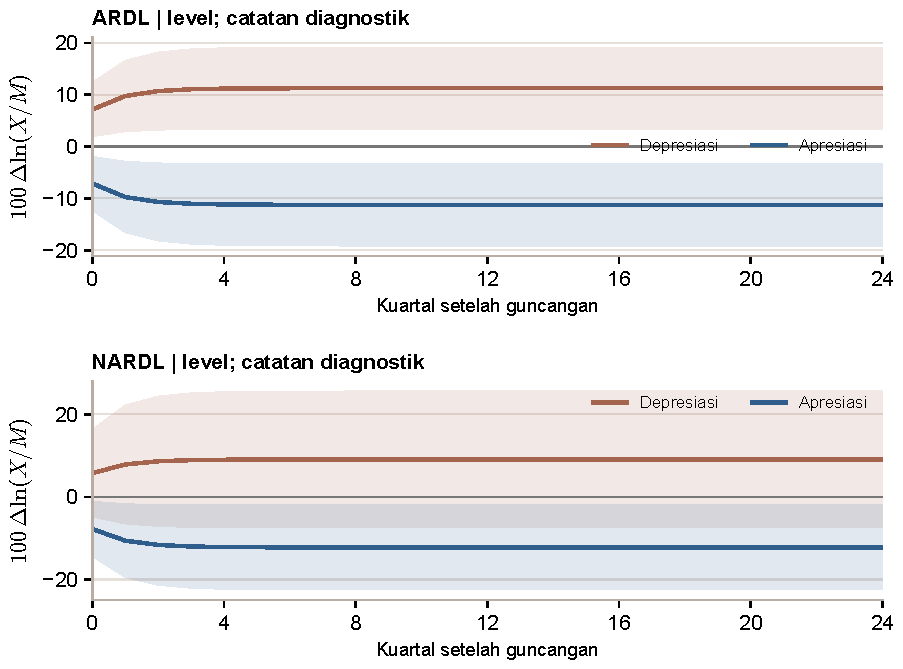
\includegraphics[width=\linewidth]{assets/response_BIL_THA.pdf}\caption{Respons perdagangan Indonesia--Thailand. Positif berarti perbaikan rasio ekspor/impor. Band pointwise nominal 95\%; skala kedua panel berbeda.}\label{fig:bilTHA}\end{figure}


\clearpage\subsection{Indonesia--Amerika Serikat}

NARDL Indonesia--Amerika Serikat memakai 75 kuartal pada 2007Q1--2025Q3. Koefisien depresiasi 3,095, CI nominal 95\% [0,921; 5,269], probabilitas nominal 0,006, dan BH 0,020. Probabilitas asimetri jangka panjang 0,240. Pemeriksaan yang membatasi: joint-X belum menolak; catatan diagnostik residual/stabilitas.

AS menghasilkan koefisien depresiasi NARDL yang positif dan signifikan nominal maupun BH. F dan t bounds juga menolak. Namun joint-X sekitar 0,060 belum melewati ambang lima persen, sehingga syarat level tambahan tidak terpenuhi. CUSUMSQ dan normalitas residual memberi catatan lain.

Sampel berhenti pada 2025Q3 akibat kekosongan CPI Oktober 2025 pada keluarga utama. Kelompok konsumsi dengan AS mempunyai dukungan berbeda dan memperlihatkan pola J yang lebih jelas. Hal tersebut tidak menyelesaikan kekurangan model total, karena agregasi barang dan persamaan yang diuji berbeda.

\begin{figure}[!htbp]\centering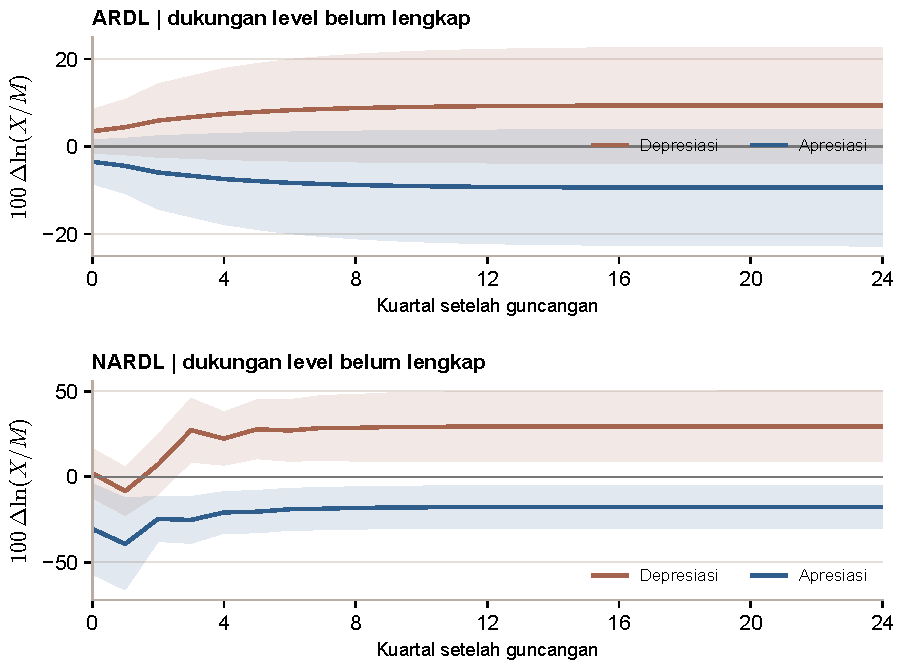
\includegraphics[width=\linewidth]{assets/response_BIL_USA.pdf}\caption{Respons perdagangan Indonesia--Amerika Serikat. Positif berarti perbaikan rasio ekspor/impor. Band pointwise nominal 95\%; skala kedua panel berbeda.}\label{fig:bilUSA}\end{figure}


\clearpage\subsection{Indonesia--Vietnam}

NARDL Indonesia--Vietnam memakai 74 kuartal pada 2007Q1--2025Q2. Koefisien depresiasi -0,551, CI nominal 95\% [-3,806; 2,704], probabilitas nominal 0,737, dan BH 0,810. Probabilitas asimetri jangka panjang 0,163. Pemeriksaan yang membatasi: F/t bounds belum menolak; catatan diagnostik residual/stabilitas.

Vietnam mempunyai catatan varians dan stabilitas yang cukup luas. NARDL memberikan koefisien depresiasi negatif yang tidak signifikan, sedangkan t bounds belum mendukung keputusan level. ARDL juga belum memenuhi seluruh syarat dan menolak beberapa diagnostik. Koefisien tidak dipilih hanya karena arahnya sesuai atau bertentangan dengan hipotesis.

Kekosongan kurs Agustus 2025 memotong jendela utama yang lengkap pada 2025Q2. Prosedur tidak merapatkan kuartal setelah celah dan menganggapnya berurutan. Alternatif GEM tetap merupakan sensitivitas dengan konsep sumber yang mungkin berbeda. Keterbatasan itu memengaruhi perbandingan Vietnam dengan mitra yang berakhir lebih akhir.

\begin{figure}[!htbp]\centering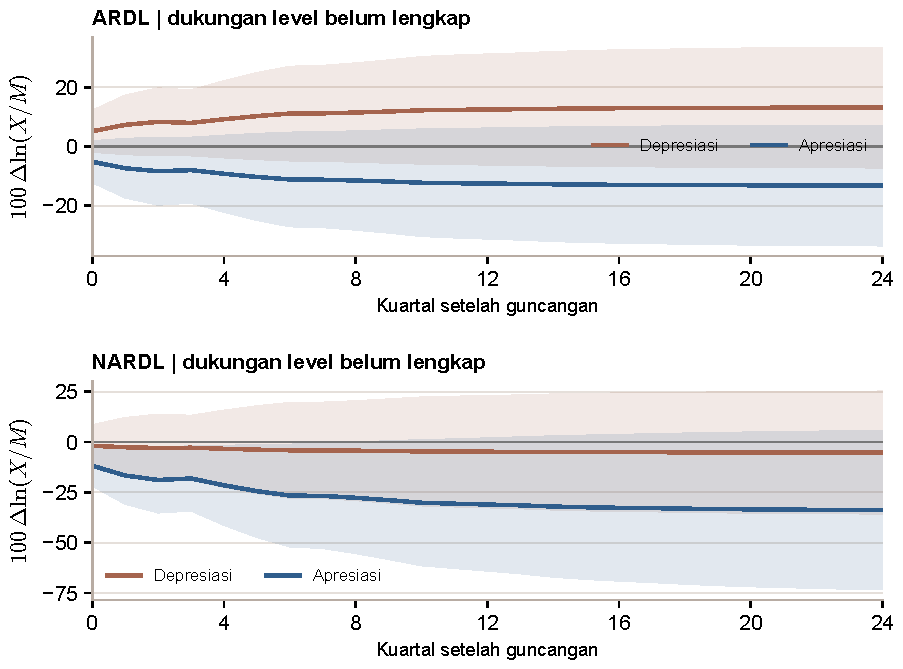
\includegraphics[width=\linewidth]{assets/response_BIL_VNM.pdf}\caption{Respons perdagangan Indonesia--Vietnam. Positif berarti perbaikan rasio ekspor/impor. Band pointwise nominal 95\%; skala kedua panel berbeda.}\label{fig:bilVNM}\end{figure}
